\documentclass[slidestop]{beamer}
\usepackage{beamerthemesplit}
\usepackage{graphics}
\usepackage{pstricks}

\title{Commercial Libre-RISCV SoC}
\author{Luke Kenneth Casson Leighton}


\begin{document}

\frame{
   \begin{center}
    \huge{Designing a Commercial Libre RISC-V SoC}\\
    \vspace{32pt}
    \Large{Ethical Strategic Leveraging of the benefits}\\
    \Large{of Libre and Open SW/HW}\\
    \Large{for pure unadulterated Commercial gain}\\
    \vspace{24pt}
    \Large{Chennai 9th RISC-V Workshop}\\
    \vspace{16pt}
    \large{\today}
  \end{center}
}


\frame{\frametitle{Credits and Acknowledgements}

 \begin{itemize}
   \item The Designers of RISC-V\vspace{15pt}
   \item The Shakti Group\vspace{15pt}
   \item Prof. G S Madhusudan\vspace{15pt}
   \item Neel Gala\vspace{15pt}
   \item Rishabh Jain\vspace{15pt}
  \end{itemize}
}


\frame{\frametitle{Why, How, What?}

 \begin{itemize}
   \item Why? Because these days it's just not necessary to
         make [un]ethical compromises in order to make a profitable,
         desirable mass-volume product\\
         {\it (There's enough companies doing that: where it's got us??)}
   \item How? By leveraging the long-establised strategic cost and
         maintenance benefits of libre-licensed software (and
         HDL) and
         {\it making sure that the people who provide it are
         financially rewarded}.  Also by empowering diverse team
         collaboration
   \item What? A 2.5ghz RISC-V 64-bit SoC that has
		 a 3D Embedded GPU, 1080p Video decode, and interfaces
		 to make it attractive for use in tablets, netbooks, industrial
		 embedded and more.  22nm or less, under 400 pins, under USD \$4.\\
  {\it All sounds obvious... but is it practical and achievable?}
  \end{itemize}
}


\frame{\frametitle{Definitions}

 \begin{itemize}
   \item {\bf Business}: the provision of a service and being
		 commensurately financially rewarded for doing so
   \item {\bf Spongeing}: the provision of a service and being
		  taken advantage of for doing so {\it (cf: Professor Yunus)}
	\item {\bf An ethical act}: an act that increases truth,
		  love, awareness or creativity for one or more people
		  (including yourself), {\it without} reducing those
		  same four qualities {\it for anyone}
	\item {\bf The Four Freedoms}: the rights and guarantees
		  associated with and embedded within GNU Licenses {\it (cf: FSF)}
  \end{itemize}
  {\it Is it possible to ethically do business and respect the
   Four Freedoms? That's where it gets interesting, as there are
   even cases where the Four Freedoms are unethical.  Note: google's
   former motto "don't be evil" is clearly (unintentionally) unethical}
}


\frame{\frametitle{How on earth does an ethical Libre SoC make money???}

 \begin{itemize}
   \item Simple answer: Mask Rights.
   \item Without Mask Rights: by having a desirable
         product, and packaging it for a customer (i.e. by being a middle-man
         a service is still being provided for which payment etc. etc.)
   \item Without a desirable product or customer(s): err... you don't.\\
	     (cf: definition of Business)
   \item By not having high NREs (leveraging back-to-back deals,
	     and helping others fulfil their needs)
  \end{itemize}
  {\it Detachment from the goal also helps. If someone else makes this
   product then GREAT! I can go do something else}

}

\frame{\frametitle{Things wot are "off-limits"}

 \begin{itemize}
   \item Customer entrapment (through proprietary software).\\
         Strong business case for not entrapping customers:\\
	     https://tinyurl.com/most-productive-meeting-ever
   \item Funding, endorsing, empowering or otherwise supporting
	      unethical Companies, Organisations and Individuals.\\
	     (cf: definition of an ethical act).
	\item Being totally inflexible / unrealistic.  Goals have
	     to be met: it's no good being an idiot about that. If
	     a Libre 3D GPU really can't be made, use Vivante GC800
	     (with etnaviv).
  \end{itemize}
  {\it Still no real show-stoppers to making money (or product):
    it's just slightly harder, that's all.  Ultimately it's about
    confidence. }
}


\frame{\frametitle{Interfaces, Block Diagram, of the Libre-RISCV SoC}
 \begin{center}
  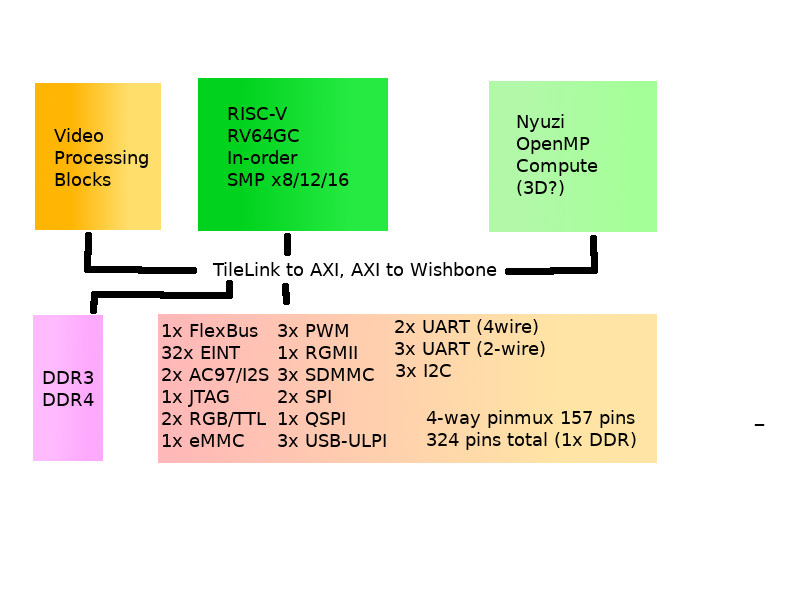
\includegraphics[height=2.1in]{../shakti_libre_riscv.jpg}\\
  {\bf Separate Power Domains for GPIO banks, Variable voltages
    required, low-power sleep states etc.  Quite involved}
 \end{center}
}

\frame{\frametitle{Hardware / Development Complexity Comparison}

 \begin{itemize}
   \item {\bf Server}: relatively easy. PCIe, RapidIO, XAUI, SATA, (1/10) GbE,
		 DDR3/4 (or HMC) etc. etc. No multiplexing: all interfaces dedicated
		 and high-speed differential pairs.
   \item {\bf Desktop}: really just a variant of Server.
	     Graphics is a PCIe Card (except if integrated).  Peripherals
	     often done in dedicated external ICs ("Southbridge" concept)
   \item {\bf Embedded}: also pretty easy.  Really needs a pinmux.  Low clock
         rate, low power mode.  e.g. SiFive Freedom U310.
   \item {\bf Mobile}: HARD. Performance/Watt matters $=>$ variable core
		 voltage domains {\it per core}.  Number of pins matters (affects
		 yield and package cost).  Cost
		 matters.  Pinmux critical.
  \end{itemize}
  {\it Bottom line: Mobile-class processors are challenging!}
}


\frame{\frametitle{TODO}

 \begin{itemize}
   \item TODO\vspace{8pt}
  \end{itemize}
}


\frame{\frametitle{Summary}

 \begin{itemize}
   \item TODO
  \end{itemize}
}


\frame{
  \begin{center}
    {\Huge The end\vspace{20pt}\\
		   Thank you\vspace{20pt}\\
		   Questions?\vspace{20pt}
	}
  \end{center}
  
  \begin{itemize}
	\item Discussion: 
	\item http://libre-riscv.org/shakti/m\_class/
  \end{itemize}
}


\end{document}
